\section{Github}

\begin{frame}
\begin{center}
\includegraphics[scale=0.2]{github-logo.png}
\includegraphics[scale=0.4]{github-logo.pdf}\end{center}
\end{frame}

\begin{frame}
\begin{quote}«~GitHub est un service web d'hébergement et de gestion de développement de logiciels, utilisant le programme Git.~»\end{quote}
\begin{flushright}--- Wikipédia\end{flushright}
\end{frame}

\begin{frame}{Concurrents}

\begin{center}
\includegraphics[scale=0.5]{sourceforge-logo.png}\end{center}

\begin{center}
\includegraphics[scale=0.1]{gitlab-logo.png}{\Huge Gitlab}\end{center}

\end{frame}

\begin{frame}{Gestion de compte}
Il est possible de définir notament :
\begin{itemize}
	\item avatar
	\item pseudo
	\item email
	\item clé SSH (important)
\end{itemize}
\end{frame}

\begin{frame}{Gestion de dépôts}
Github permet de :
\begin{itemize}
	\item Créer des dépôts (https://github.com/new)
	\item Gérer les collaborateurs sur un dépôt
	\item Suivre des dépôts
	\item Fourcher des dépôts
\end{itemize}
\end{frame}

\begin{frame}{Documentation et rapport de bugs}
\begin{itemize}
	\item README.md
	\item Gestionnaire de problèmes
	\item Site web statique (ou Jekyll)
	\item Wiki
\end{itemize}
\end{frame}

\begin{frame}{Autres services}
Gist :
\begin{itemize}
	\item https://gist.github.com/
	\item Partage de petits textes (morceux de code, …)
\end{itemize}

Travis CI :
\begin{itemize}
	\item https://travis-ci.org/
	\item Intégration continue
\end{itemize}
\end{frame}

\begin{frame}{Applications}
Il existes des applications officielles pour :
\begin{itemize}
	\item Windows
	\item Mac OS
	\item Android
\end{itemize}
\begin{center}
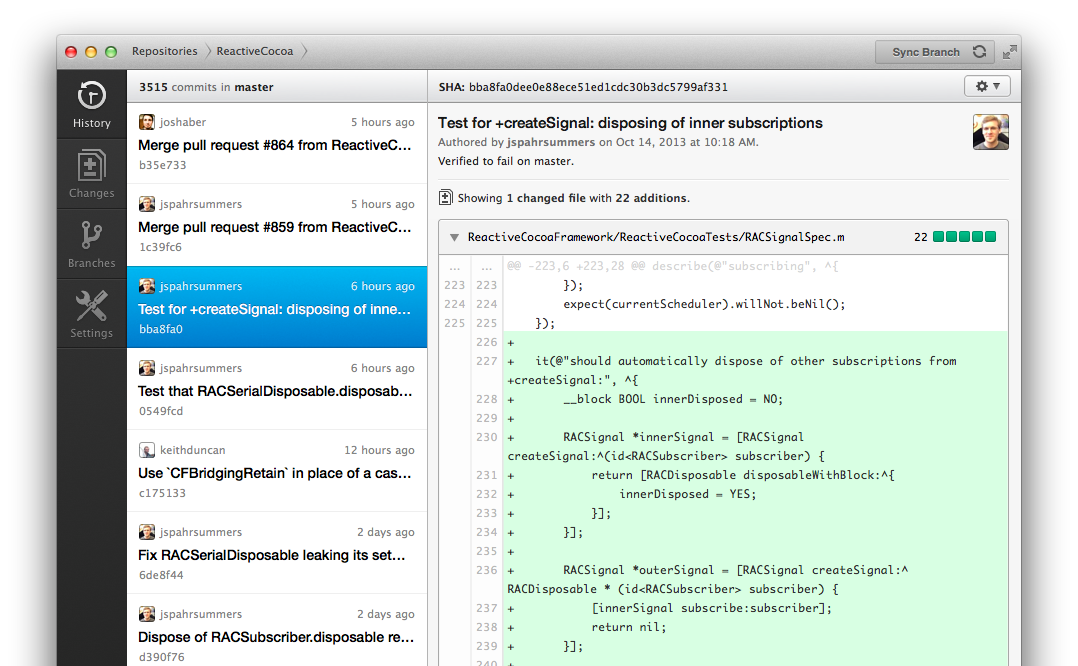
\includegraphics[scale=0.3]{screen1.png}
\end{center}
\end{frame}

